% XCircuit output "salida.tex" for LaTeX input from salida.eps
\def\putbox#1#2#3#4{\makebox[0in][l]{\makebox[#1][l]{}\raisebox{\baselineskip}[0in][0in]{\raisebox{#2}[0in][0in]{\scalebox{#3}{#4}}}}}
\def\rightbox#1{\makebox[0in][r]{#1}}
\def\centbox#1{\makebox[0in]{#1}}
\def\topbox#1{\raisebox{-0.60\baselineskip}[0in][0in]{#1}}
\def\midbox#1{\raisebox{-0.20\baselineskip}[0in][0in]{#1}}
   \scalebox{1}{
   \normalsize
   \parbox{6.61458in}{
   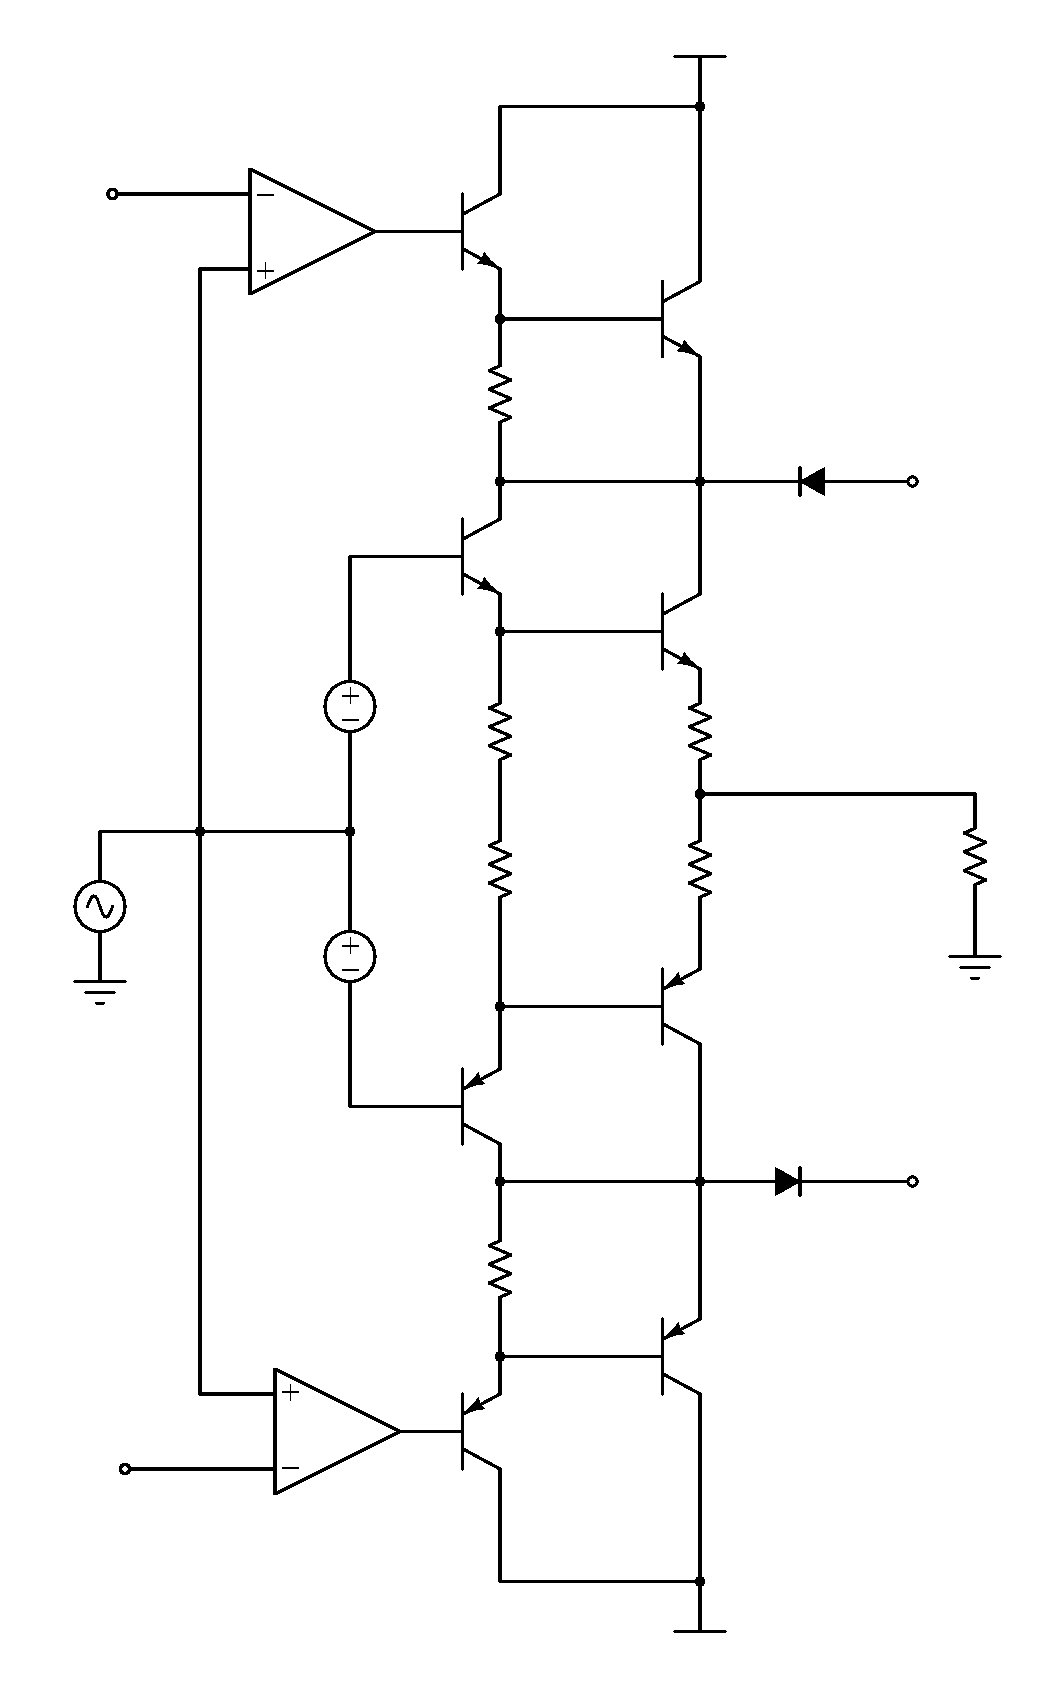
\includegraphics[scale=1]{salida}\\
   % translate x=800 y=1584 scale 0.38
   \putbox{1.39in}{6.39in}{1.20}{Vbias1}%
   \putbox{1.39in}{4.81in}{1.20}{Vbias2}%
   \putbox{5.89in}{5.39in}{1.20}{RL}%
   \putbox{4.72in}{6.22in}{1.20}{Re}%
   \putbox{4.72in}{5.31in}{1.20}{Re}%
   \putbox{4.47in}{6.89in}{1.20}{Q63}%
   \putbox{4.47in}{4.39in}{1.20}{Q64}%
   \putbox{3.14in}{7.47in}{1.20}{Q14}%
   \putbox{3.14in}{3.72in}{1.20}{Q15}%
   \putbox{3.14in}{9.56in}{1.20}{Q16}%
   \putbox{4.47in}{9.06in}{1.20}{Q62}%
   \putbox{3.14in}{1.56in}{1.20}{Q17}%
   \putbox{4.47in}{2.06in}{1.20}{Q65}%
   \putbox{0.14in}{1.31in}{1.20}{Vth-}%
   \putbox{0.06in}{9.81in}{1.20}{Vth+}%
   \putbox{4.22in}{0.06in}{1.20}{-VccH}%
   \putbox{4.22in}{10.89in}{1.20}{+VccH}%
   \putbox{6.06in}{7.89in}{1.20}{VccL+}%
   \putbox{6.06in}{3.22in}{1.20}{-VccL}%
   } % close 'parbox'
   } % close 'scalebox'
   \vspace{-\baselineskip} % this is not necessary, but looks better
